\chapter[Experimentos e Resultados]{Experimentos e Resultados} \label{cap:resultados}
    Para testar o pacote \textit{rqt\_mrta}, será necessário uma arquitetura desenvolvida sobre o \textit{framework} ROS. Primeiramente, será necessário compreendê-la e entender como parametrizá-la. A partir disso, será possível estruturar os \textit{templates} de arquivos de configuração e de inicialização, isto é, criar seu arquivo de configuração, conforme descrito em \ref{subsec:arch_config_fmt}. Tendo este arquivo em mãos, é preciso alterar o arquivo manifesto do seu pacote para que a configuração possa ser vista pelo \textit{rqt\_mrta}. Este processo foi descrito em \ref{subsec:arch_config_rgst}. Finalmente, a arquitetura estará cadastrada e pronta para ser configurada por usuários na criação de aplicações.
    
    Além de uma arquitetura, será necessário a elaboração de uma aplicação que utilize a arquitetura cadastrada. Pois, assim, será validado o processo de criação da aplicação. Isto é, deverá ser verificado se o pacote da nova aplicação foi gerado com sucesso. Para isso, deve se verificar se ele é visível pelas ferramentas de busca do ROS e se a formatação dos arquivos de parâmetro, de inicialização e de configuração de aplicação está correta. Se tudo estiver em conformidade, então a aplicação estará pronta para a execução. É preciso, agora, executar a aplicação utilizando os arquivos de inicialização gerados pelo \textit{rqt\_mrta}. Para isso, será utilizada a ferramenta \textit{roslaunch} para a inicialização dos nós da aplicação. 
    
    Finalmente, será verificado o sistema supervisório do \textit{rqt\_mrta}. Para isso, a aplicação deverá ser carregada pelo \textit{rqt\_mrta}, o qual ficará aguardando a aplicação ser executada. Nesta etapa será verificada a alteração do estado dos robôs no sistema e, se fornecido, a inicialização do \textit{plugin} para o monitoramento da arquitetura.
    
    Pelo fato de haver poucas aproximações genéricas de arquitetura MRTA para aplicações baseadas em ROS, foi desenvolvido o pacote \textit{alliance}. Esse pacote faz uma aproximação independente do domínio da arquitetura tolerante a falhas ALLIANCE \cite{ref:parker1998alliance} para atribuição de tarefa em sistema multirrobô. Esta arquitetura será utilizada para testar o funcionamento do pacote \textit{rqt\_mrta}. 
    
    Será criado, através do \textit{rqt\_mrta}, uma aplicação que utilize a arquitetura desenvolvida no pacote \textit{alliance} para a atribuição de tarefa no sistema. Será simulado a patrulha realizada por múltiplos robôs.
    
    Será descrito a seguir o desenvolvimento da arquitetura ALLIANCE no pacote \textit{alliance}. Em seguida, está arquitetura será cadastrada para sua utilização por aplicações no \textit{rqt\_mrta}. Depois, a aplicação será explicada e criada através do \textit{rqt\_mrta}. Por fim, os arquivos de inicialização da arquitetura serão executados em conjunto com o simulador e os demais nós para a execução da aplicação.

    \section{\textit{alliance}} \label{sec:alliance}
        O \textit{alliance} é um projeto baseado em ROS que contém nós que fazem o controle distribuído da alocação de tarefa em um sistema com múltiplos robôs segundo o modelo sugerido por \citeonline{ref:parker1998alliance}, a arquitetura ALLIANCE. Esta arquitetura resolve problema do tipo \textit{ST-SR-IA}, ou seja, cada robô do sistema só pode executar uma tarefa por vez, as tarefas requisitadas só podem ser executadas por um único robô e atribuição das tarefas ocorre instantaneamente, não sendo considerado o estado do sistema no futuro.
        
        Esta abordagem é baseada em comportamento. Cada robô do sistema possui diversos comportamentos. A ativação de um dado comportamento faz com que o robô passe a executar uma tarefa específica. Assim, uma nova alocação acontece sempre que um robô muda de comportamento. 
        
        Cada configuração de comportamento nos robôs possui um mecanismo para o cálculo de motivação que cresce em função de várias variáveis. Quando o nível de motivação de um dado comportamento atinge seu limite, este é ativado. As duas variáveis principais são impaciência e aquiescência. A impaciência do robô aumenta o nível de motivação em função das atividades dos demais robôs do sistema. Porém, a aquiescência leva o nível de motivação para zero, quando o robô verifica que ele deve desistir da tentativa de executar a tarefa especificada pelo comportamento. O Apêndice \ref{app:alliance} dá mais detalhes sobre o funcionamento da arquitetura ALLIANCE.
        
        Este pacote possui dois nós: \textit{high\_level} e \textit{low\_level}. Cada robô do sistema deve rodar esses dois nós para o bom funcionamento da arquitetura. Não são necessários nós adicionais, no que diz respeito à alocação de tarefa. O nó \textit{high\_level}, possui um nível de abstração maior, pois ele controla a ativação do comportamento a partir da análise do estado do sistema. Este nó possui diversos parâmetros, os quais afetam diretamente no desempenho do sistema. Pois estes parâmetros ditam a dinâmica da motivação de comportamento de um dado robô do sistema. Enquanto isso, o nó \textit{low\_level}, possui uma abstração mais baixa, pois este interage diretamente com o nível de controle de execução de tarefa. Este nó desempenha o papel de cuidar da análise sensorial dos comportamentos do robô e, ainda, direcionar para o nível de controle da execução da tarefa qual tarefa deve ser executada.
        
        O nó \textit{low\_level} demanda maior detalhamento, pois ele é altamente dependente de implementações realizadas pelos usuários do pacote \textit{alliance}. Para que fosse possível uma aproximação genérica do ALLIANCE, isto é, que pudesse ser utilizada em qualquer aplicação que atende as premissas desta arquitetura, utilizou-se o pacote \textit{pluginlib}\footnote{\url{http://wiki.ros.org/pluginlib}}. Este pacote contém uma biblioteca C++ para carregar e descarregar \textit{plugins} de pacotes do ROS. \textit{Plugins} são classes dinamicamente carregáveis que são carregadas de uma biblioteca externa em tempo de execução. Desta forma, o usuário pode fazer a análise sensorial e desenvolver a camada de controle de execução de tarefa de forma a atender a sua aplicação. Para isso foram criadas as seguintes classes base: \textit{alliane::Sensor}, \textit{alliance::SensoryEvaluator} e \textit{alliance::Layer}. Será explicado a seguir sobre o desenvolvimento de \textit{plugins} de sensor, avaliação e camada, mostrando o cabeçalho em C++ da classe base de cada tipo de \textit{plugin}.
        
        \lstset{language=C++,
                numbers=left,
                stepnumber=1,
                basicstyle=\ttfamily,
                keywordstyle=\color{blue}\ttfamily,
                stringstyle=\color{red}\ttfamily,
                commentstyle=\color{green}\ttfamily,
                morecomment=[l][\color{magenta}]{\#}
        }
        
        \subsection{\textit{Plugin} de sensor} \label{subsec:alliance_sensor}
            A classe \textit{alliance::Sensor} permite que o usuário do \textit{alliance} desenvolva \textit{plugins} de sensores reais ou virtuais. O usuário tem a flexibilidade de se inscrever em qualquer tópico do ROS para fazer leitura dos sensores cujos sinais são publicados por outros nós. Ou ainda pode ser utilizadas técnicas de fusão sensorial, filtragem e conversões para melhorar a análise sensorial. Mas, também, é possível criar sensores virtuais que utilizam temporizadores ou avaliam o estado abstrato das entidades do sistema. Os \textit{plugins} dos sensores são estipulados na inicialização do nó \textit{low\_level} por meio de parâmetros do ROS. Se o \textit{plugin} desenvolvido pelo usuário estiver devidamente cadastrado (conforme descrito na página do pacote \textit{pluginlib}), o nó \textit{low\_level} não haverá problemas para carregá-lo. Por fim, é importante salientar que o usuário pode especificar diversos \textit{plugins} de sensor.
            
            \lstinputlisting{Outros/Arquivos/4_resultados/sensor.h}
            
            O \textit{plugin} deve sobre-escrever o método \textit{initialize} para que ele possa ser inicializado corretamente. Será disponibilizado à ele o \textit{namespace} do nó \textit{low\_level}, o nome e o \textit{id} do sensor. Porém, o \textit{plugin} pode ser configurado através da leitura de parâmetros do ROS. Para uma melhor organização, é aconselhável sobre-escrever o método \textit{readParameters} para fazer isso. Pois, a classe \textit{alliance::Sensor} já chama este método logo após a inicialização do \textit{plugin}. Enfim, o \textit{plugin} pode sobre-escrever o método \textit{isUpToDate} para informar se os dados providos do sensor real estão sendo recebidos. 
            
            Foi criada uma classe utilitária genérica, denominada \textit{nodes::ROSSensorMessage}, para simplificar o trabalho do usuário do \textit{alliance}. Está classe herda os métodos da classe \textit{alliance::Sensor} e, assim, também pode ser usada como classe base para criação de \textit{plugins} de sensor. Diferentemente da classe \textit{alliance::Sensor}, a classe \textit{nodes::ROSSensorMessage} se inscreve no tópico que transporta mensagens contendo o sinal do sensor desejado. Neste caso, o \textit{id} do sensor é considerado como o nome deste tópico. Esta classe sobre-escreve o método \textit{readParameters} para coletar parâmetros que são utilizados no método \textit{isUpToDate}, o qual é sobre-escrito para identificar se a última mensagem foi recebida dentro do tempo máximo especifidado. Assim, os \textit{plugins} que se baseiam nesta classe terão a última mensagem recebida disponível para a sobre-escrita do método \textit{isApplicable}.
        
        \subsection{\textit{Plugin} de avaliação sensorial} \label{subsec:alliance_evaluator}
            A classe base \textit{alliance::SensoryEvaluator} tem como responsabilidade analisar os sensores estipulados em uma dada configuração de comportamento. Através dessa análise este avaliador enviará uma mensagem ao nó \textit{high\_level} dizendo se ativação deste comportamento específico é aplicável ou não. Como esta análise sensorial varia de uma aplicação para outra, essa classe foi projetada para a criação de \textit{plugins} de avaliação. Através do recurso de herança do C++, o método \textit{isApplicable} deve ser implementado pelo \textit{plugin}, onde deverá ser realizada a análise sensorial. Para isso, este objeto terá disponível a coleção de \textit{plugins} de sensor devidamente carregados para a análise. O \textit{plugin} é inicializado através da sobre-escrita do método \textit{initialize}, onde são dados: (1) um objeto \textit{ros::NodeHandlePtr} para a interação com o ROS, (2) o objeto robô que contém a instância de todos os sensores, (3) a tarefa sobre o qual é feita a análise e, também, (4) uma lista com os \textit{ids} dos sensores que devem ser considerados durante a análise.
            
            \lstinputlisting{Outros/Arquivos/4_resultados/sensory_evaluator.h}
        
        \subsection{\textit{Plugin} de camada} \label{subsec:alliance_layer}
            Os \textit{plugins} criados a partir da classe base \textit{alliance::Layer} têm como responsabilidade controlar a execução da tarefa pelo robô. O usuário deve criar um \textit{plugin} de camada para cada tarefa. Entretanto, se houver robôs que executam uma mesma tarefa de modos diferentes, cada modo terá seu próprio \textit{plugin}. Como o nome da classe base sugere, o usuário tem a flexibilidade de implementar esses \textit{plugins} em camadas, conforme sugerido por \cite{ref:parker1998alliance}.
            
            \lstinputlisting{Outros/Arquivos/4_resultados/layer.h}
            
            O \textit{plugin} de camada é inicializado através da chamada do método \textit{initialize}. Logo, este método deve ser sobre-escrito na classe do \textit{plugin}, onde será disponibilizado o \textit{namespace} do seu nó, bem como, o nome da camada. Porém, o \textit{plugin} pode ser configurado a partir da leitura de parâmetros do ROS. Para uma melhor organização, é recomendado que esta leitura seja realizada dentro da sobre-escrita do método \textit{readParameters}, pois a classe \textit{alliance::Layer} faz sua chamada logo após a inicialização do \textit{plugin}. Finalmente, o controle da execução da tarefa é realizado periodicamente através da sobre-escrita do método \textit{process}. Este método deve ser utilizado para atualizar os sinais de comando dos atuadores do robô.
            
            Verifica-se que o desenvolvimento desta aproximação do ALLIANCE é genérica e possui uma API simplificada. Deste modo, o usuário pode focar no desempenho dos robôs na execução das tarefas.
        
        \subsection{\textit{alliance\_msgs}}
            O pacote \textit{alliance\_msgs} foi criado em conjunto com o pacote \textit{alliance} para separar as definições dos tipos de mensagens utilizadas por ele. Essas mensagens são utilizadas na comunicação entre os nós do pacote \textit{alliance}.
            
            Este pacote define as seguintes mensagens:
            
            \begin{itemize}
                \item \textit{alliance\_msgs/InterRobotCommunication}: armazena informação sobre a atividade de um robô específico em um dado instante. Possui o cabeçalho padrão do ROS que identifica o robô que enviou a mensagem e instante que ela foi enviada. Além disso, ela possui um campo que identifica a tarefa que o robô está executando;
                \item \textit{alliance\_msgs/Motivation}: utilizada para o monitoramento da arquitetura. Esta mensagem possui o cabeçalho padrão do ROS para identificar o robô que a enviou e também o instante em que ela foi enviada. Além disso, ela possui um campo que identifica a tarefa que o cálculo de motivação se referencia e, ainda, o valor das variáveis que influenciam no cálculo da motivação;
                \item \textit{alliance\_msgs/SensoryFeedback}: utilizada na comunicação entre os nós de baixo e alto nível de abstração de um mesmo robô. Esta mensagem informa se um dado comportamento é aplicável em um dado instante segundo uma análise sensorial realizada no nível de baixa abstração do \textit{alliance}. Logo, esta mensagem possui o cabeçalho padrão do ROS que identifica o robô que a enviou e o instante em que ela foi enviada. Além disso, ela possui um campo que identifica a tarefa sobre a qual a análise é referenciada e, ainda, um campo informando se a ativação do comportamento que leva esse robô à execução dessa tarefa é aplicável.
            \end{itemize}
        
        \subsection{\textit{rqt\_alliance}}
            O pacote \textit{rqt\_alliance} foi desenvolvido para auxiliar no monitoramento da arquitetura implementada no pacote \textit{alliance}. Ele fornece uma ferramenta gráfica que detalha as variáveis que influenciam no cálculo de motivação de uma dada configurações de comportamento de um robô específico. Este \textit{plugin} também fornece gráficos que mostram o nível de motivação para a ativação de cada comportamento de um dado robô.
            
            A Figura \ref{fig:rqt_alliance_detailed_motivation} detalha graficamente o cálculo da motivação da configuração de comportamento que leva o robô \textit{/robot2} executar a tarefa \textit{wander}. De cima para baixo estão os seguintes gráficos: (1) nível de motivação, (2) taxa de impaciência, (3) aquiescente, (4) suprimido, (5) reiniciada, (6) aplicável e (7) ativa. Perceba que o comportamento se mantém ativo (gráfico mais abaixo) enquanto o nível de motivação (linha contínua azul do gráfico mais acima) é igual ou superior ao \textit{threshold} (linha tracejada vermelha do gráfico mais acima). Note que no instante em que o robô se tornou aquiescente (impulso visto no terceiro gráfico de cima para baixo), o nível da sua motivação para ativar o comportamento \textit{wander} é zerado. O nível de motivação é zerado também, ao final, quando esse comportamento se torna inaplicável. As demais variáveis permanecem constante durante todo o intervalo.
            
            \begin{figure}
                \centering
                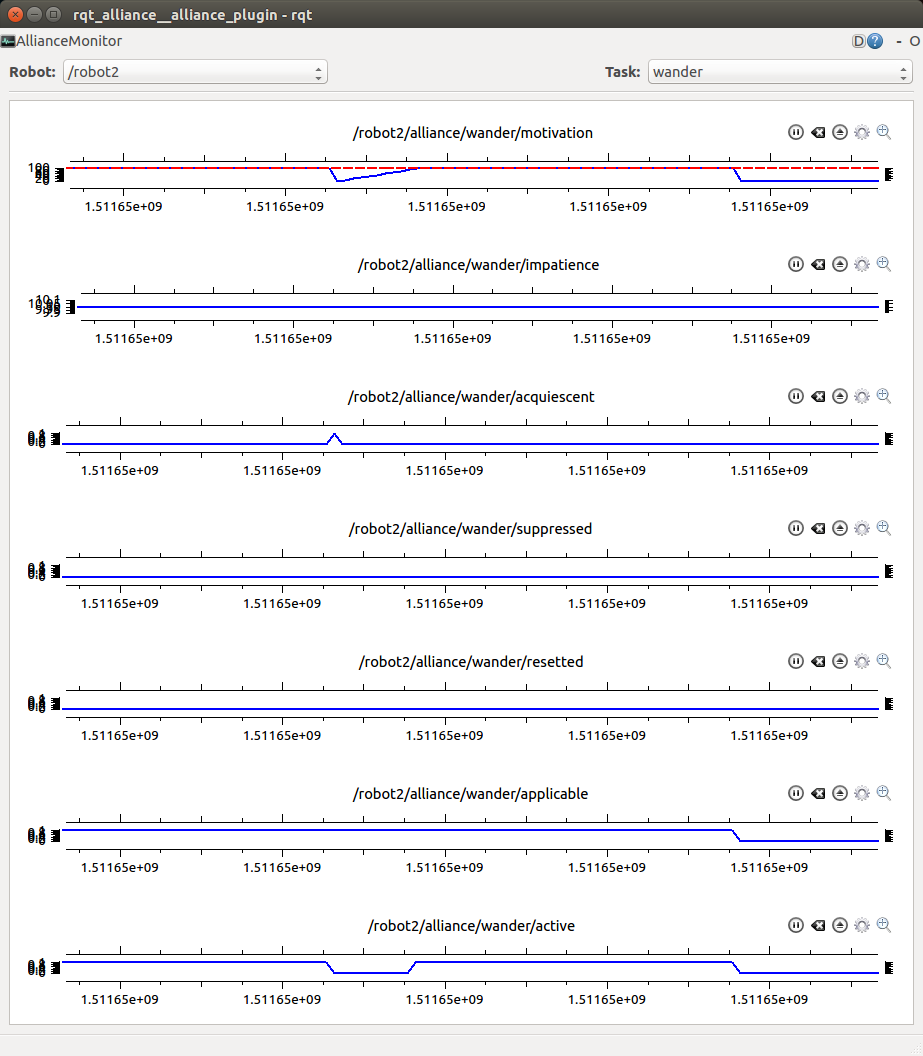
\includegraphics[width=\textwidth]{Figuras/4_resultados/rqt_alliance6.png}
                \caption{Detalhamento da motivação \textit{/robot2/alliance/wander} ao longo do tempo.}
                \label{fig:rqt_alliance_detailed_motivation}
            \end{figure}
            
            A Figura \ref{fig:rqt_alliance_motivations}, por exemplo, mostra que o robô \textit{/robot3} possui três configurações de comportamento: (1) \textit{wander}, (2) \textit{border\_protection} e (3) \textit{report}. Nesta figura, é mostrado o nível de motivação do robô \textit{/robot3} para cada um dos comportamentos ao longo do tempo. Uma dada configuração de comportamento é ativada quando sua motivação (linha contínua azul) atinge o \textit{threshold} (linha tracejada vermelha). Note que, enquanto o comportamento \textit{report} do robô \textit{/robot3} não está ativo, há um aumento na motivação de todos os seus comportamentos. Porém, em ambos casos, a motivação de \textit{report} atinge o \textit{threshold} antes das outras. Isso se deve pelo fato dessa motivação de comportamento apresentar uma dinâmica mais rápida que as demais. Isso não significa que o robô \textit{/robot3} executará somente a tarefa \textit{report}. Dependendo do estado do sistema, outro robô pode passar a realizá-la em seu lugar.
            
            \begin{figure}
                \centering
                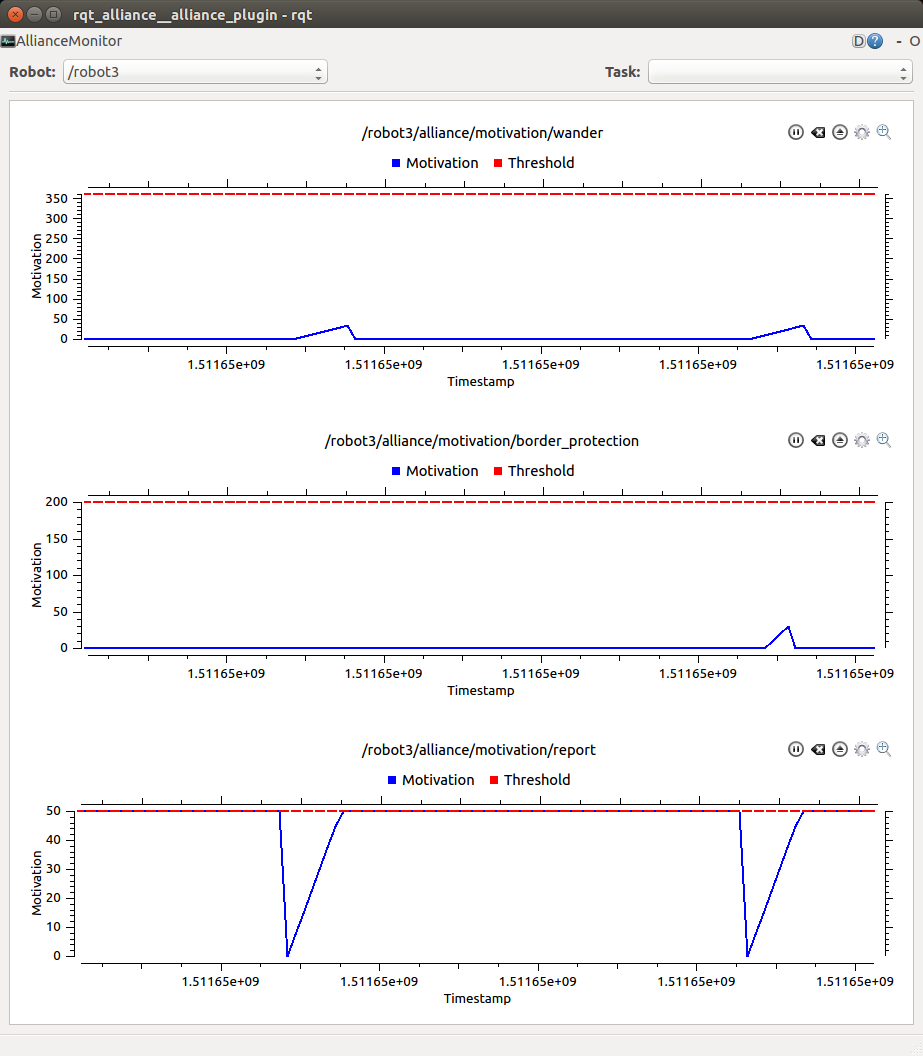
\includegraphics[width=\textwidth]{Figuras/4_resultados/rqt_alliance4.png}
                \caption{Motivações das configurações de comportamento do robô \textit{/robot3}.}
                \label{fig:rqt_alliance_motivations}
            \end{figure}
            
        \subsection{Arquivos de parâmetro do \textit{alliance}} \label{subsec:alliance_config}
            Os nós \textit{high\_level} e \textit{low\_level} do pacote \textit{alliance} são configurados a partir da leitura de parâmetros do ROS durante a inicialização. 
            
            Existem três tipos de arquivos de parâmetro no \textit{alliance}: de camada, de tarefa e de robô. O arquivo de parâmetro de camada traz configurações pertinentes para a execução das tarefas. Por este fato, este arquivo não é definido pelo pacote \textit{alliance}. O arquivo de parâmetros de tarefa especifica quais são as tarefas existentes no sistema. Um exemplo deste arquivo é exibido a seguir.
            
            \lstset{language=Python,
                keywords={true,false,null,y,n},
                keywordstyle=\color{black}\bfseries,
                ndkeywords={},
                ndkeywordstyle=\color{black}\bfseries,
                identifierstyle=\color{black},
                sensitive=false,
            }
            
            \begin{lstlisting}
                tasks:
                  size: 3
                  task0:
                    id: wander
                    name: Wander
                    layers:
                      size: 1
                      layer0:
                        plugin_name: alliance_test/wander
                  task1:
                    id: border_protection
                    name: Border Protection
                    layers:
                      size: 1
                      layer0:
                        plugin_name: alliance_test/border_protection
                  task2:
                    id: report
                    name: Report
                    layers:
                      size: 1
                      layer0:
                        plugin_name: alliance_test/report
            \end{lstlisting}
            
            Cada robô deve informar quais sensores e configurações de comportamento ele possui. Cada configuração é parametrizada de acordo com a dinâmica de ativação desejada.
            
            \begin{lstlisting}
                name: Robot 1
                spin_rate: 2.0           # in Hertz
                broadcast_rate: 0.5      # in Hertz
                timeout_duration: 10.0    # in seconds
                buffer_horizon: 10.0      # in seconds
                sensors:
                  size: 1
                  sensor0:
                    plugin_name: alliance_test/point_cloud
                    topic_name: sonar
                    timeout_duration: 5.0
                    buffer_horizon: 5.0
                behaviour_sets:
                  size: 1
                  behaviour_set0:
                    task_id: wander
                    task_expected_duration: 100.0 # in seconds
                    motivational_behaviour:
                      threshold: 150.0
                      acquiescence:
                        yielding_delay: 75.0    # in seconds
                        giving_up_delay: 110.0  # in seconds
                      impatience:
                        fast_rate: 5.0
                      sensory_feedback:
                        plugin_name: alliance_test/updated_sensory
                        sensors:
                          size: 1
                          sensor0:
                            topic_name: sonar
            \end{lstlisting}
            
        \subsection{Arquivo de inicialização do \textit{alliance}} \label{subsec:alliance_launch}
            O pacote \textit{alliance} possui apenas um arquivo de inicialização. Este arquivo carrega os arquivos de parâmetros de tarefa e de robô para o nó \textit{high\_level} e os de tarefa, de robô e de camada para o nó \textit{low\_level}. Este arquivo deve ser utilizado para cada robô do sistema, cada um especificando os seus arquivos de parâmetros. Ele é mostrado a seguir.
            
            \lstset{
                language=XML,
                breaklines=true,
                frameround=ffff,
                frame=single,
                rulecolor=\color{black},
                autogobble=true,
                morekeywords={
                    xml, version,
                    launch,
                        arg, name, value, default,
                        group, ns,
                        node, name, pkg, type, output,
                        param, name, type, value,
                        rosparam, file, command
                }
            }
            
            \begin{lstlisting}
                <?xml version="1.0"?>
                <launch>
                  <arg name="robot_id" />
                  <arg name="robot_params" />
                  <arg name="tasks_params" />
                  <arg name="layers_params" />
                  <group ns="$(arg robot_id)">
                    <group ns="alliance">
                      <node name="high_level" pkg="alliance" type="high_level" output="screen">
                        <param name="id" type="string" value="$(arg robot_id)" />
                        <rosparam file="$(arg robot_params)" command="load" />
                        <rosparam file="$(arg tasks_params)" command="load" />
                      </node>
                      <node name="low_level" pkg="alliance" type="low_level" output="screen">
                        <param name="id" type="string" value="$(arg robot_id)" />
                        <rosparam file="$(arg robot_params)" command="load" />
                        <rosparam file="$(arg tasks_params)" command="load" />
                        <rosparam file="$(arg layers_params)" command="load" />
                      </node>
                    </group>
                  </group>
                </launch>
            \end{lstlisting}
            
        \subsection{Cadastro da arquitetura do pacote \textit{alliance}}
            Primeiramente, é preciso criar o arquivo de configuração de arquitetura do pacote \textit{alliance}. Para o preenchimento completo da \textit{tag architecture}, as seguintes informações são pertinentes:
            
            \begin{itemize}
                \item a arquitetura ALLIANCE resolve problemas MRTA em que os robôs, as tarefas e as alocações são do tipo \textit{ST}, \textit{SR} e \textit{IA}, respectivamente;
                
                \item esta aproximação foi desenvolvida de modo que os robôs publicam suas atividades no tópico \textit{/alliance/inter\_robot\_communication}. O tipo de mensagem transportada por este tópico é \textit{alliance\_msgs/InterRobotCommunication}. Seus campos \textit{header/frame\_id} e \textit{task\_id} identificam, respectivamente, o robô que enviou a mensagem e a tarefa que ele estava executando no instante em que ela foi enviada;
                
                \item e, além disso, devem ser gerados para cada robô do sistema um arquivo de parâmetros e um arquivo de inicialização.
            \end{itemize}
            
            Com isso, tem-se:
            
            \lstset{
                language=XML,
                basicstyle=\ttfamily,
                keywordstyle=\color{black}\bfseries,
                ndkeywords={},
                ndkeywordstyle=\color{black}\bfseries,
                identifierstyle=\color{black},
                stringstyle=\color{red}\ttfamily,
                commentstyle=\color{green}\ttfamily,
                breaklines=true,
                frameround=ffff,
                frame=single,
                rulecolor=\color{black},
                autogobble=true,
                morekeywords={
                    xml, encoding,
                    package, format,
                    name,
                    version,
                    description,
                    maintainer, email,
                    author,
                    license,
                    url, type,
                    buildtool_depend,
                    build_depend,
                    run_depend,
                    export,
                        metapackage,
                        plugin,
                        rqt_gui,
                        alliance,
                        rqt_mrta, application, architecture,
                    xml, version, encoding,
                        rqt_mrta, format,
                            architecture,
                                name,
                                robots,
                                    busy_robots,
                                    idle_robots,
                                    config_id,
                                    launch_id,
                                    robot_0,
                                    robot_1,
                                tasks,
                                    incoming_tasks,
                                    task_0,
                                    task_1,
                                allocations,
                                    allocated_tasks,
                                    type,
                                    topic,
                                        name,
                                        type,
                                        field,
                                        timeout,
                                        queue_size,
                            configs,
                                config_0,
                                    id,
                                    value,
                                    param_0,
                                    param_1,
                                    params_0,
                                    params_1,
                                    params_2,
                                    params_3,
                                    params_4,
                                    params_5,
                                    params_6,
                                    array_0,
                                    array_1,
                                        tool_tip,
                            launches,
                                launch_0,
                                launch_1,
                                includes,
                                    include_0,
                                    include_1,
                                        file,
                                        args,
                                            arg_0,
                                            arg_1,
                                            arg_2,
                                            arg_3,
                            widgets,
                                widget_0,
                                    plugin_name,
                }
            }
            
            \begin{lstlisting}
              <architecture>
                <name>ALLIANCE</name>
                <robots>
                  <type>ST</type>
                  <busy_robots>
                    <topic>
                      <name>/alliance/inter_robot_communication</name>
                      <type>alliance_msgs/InterRobotCommunication</type>
                      <field>header/frame_id</field>
                      <queue_size>10</queue_size>
                      <timeout>2.0</timeout>
                    </topic>
                  </busy_robots>
                  <config_id>alliance_params</config_id>
                  <launch_id>alliance</launch_id>
                </robots>
                <tasks>
                  <type>SR</type>
                </tasks>
                <allocations>
                  <type>IA</type>
                  <allocated_tasks>
                    <topic>
                      <name>/alliance/inter_robot_communication</name>
                      <type>alliance_msgs/InterRobotCommunication</type>
                      <field>task_id</field>
                      <queue_size>10</queue_size>
                      <timeout>0.5</timeout>
                    </topic>
                  </allocated_tasks>
                </allocations>
              </architecture>
            \end{lstlisting}
            
            Para que os arquivos de parâmetros sejam gerados corretamente, é importante representar os padrões existentes em cada um deles através das \textit{tags param}, \textit{params} e \textit{array}. A cada avanço de \textit{namespace} foi utilizada a \textit{tag params} para agrupar um conjunto de parâmetros e a \textit{tag array} foi utilizada sempre que identificado um padrão de repetição. Nisso, foram criados os seguintes \textit{templates} de arquivos de parâmetros: 
            
            \begin{itemize}
                \item \textit{alliance\_params}: \textit{template} de robô, a partir deste modelo serão gerados arquivos de parâmetros para cada robô do sistema;
                
                \item \textit{tasks\_params}: \textit{template} de tarefas, a partir deste modelo será gerado apenas um arquivo de parâmetro referente aos dados das tarefas existentes no sistema;
                
                \item \textit{layers}: será solicitado ao usuário a inserção deste arquivo de parâmetros, já que ele não possui um modelo.
            \end{itemize}
            
            Para representar o \textit{template} do arquivo de inicialização do \textit{alliance}, foram associados todos os arquivos de parâmetros com o nome do argumento apropriado. De modo que, se obteve a seguinte representação:
            
            \begin{lstlisting}
              <launches>
                <launch_0>
                  <id>alliance</id>
                  <includes>
                    <include_0>
                      <file>$(find alliance)/launch/alliance.launch</file>
                      <args>
                        <arg_0>
                          <name>robot_id</name>
                          <value>@robot_id@</value>
                        </arg_0>
                        <arg_1>
                          <name>robot_params</name>
                          <value>$(find @package@)/config/@robot_id@_alliance_params.yaml</value>
                        </arg_1>
                        <arg_2>
                          <name>tasks_params</name>
                          <value>$(find @package@)/config/tasks_alliance_params.yaml</value>
                        </arg_2>
                        <arg_3>
                          <name>layers_params</name>
                          <value>$(find @package@)/config/layers_alliance_params.yaml</value>
                        </arg_3>
                      </args>
                    </include_0>
                  </includes>
                </launch_0>
              </launches>
            \end{lstlisting}
            
            O recurso de substituição da identificação do robô (pela palavra-chave \textit{@robot\_id@}) e o nome do pacote da aplicação (pela palavra-chave \textit{@package@}) fornecido pelo \textit{rqt\_mrta}, aumenta as possibilidades de generalidade na construção dos arquivos de inicialização.
            
            Finalmente, é identificado o nome do \textit{plugin rqt\_alliance} fornecido pela arquitetura para o monitoramento do ALLIANCE em tempo de execução. A seguinte representação foi utilizada:
            
            \begin{lstlisting}
              <widgets>
                <widget_0>
                  <plugin_name>rqt_alliance/alliance_plugin</plugin_name>
                </widget_0>
              </widgets>
            \end{lstlisting}
            
            Assim, foi obtido o arquivo de configuração da arquitetura MRTA do pacote \textit{alliance}. O arquivo completo criado pode ser visto no Apêndice \ref{app:arch_config}.
            
            Para finalizar o cadastro da arquitetura do pacote \textit{alliance} é necessário realizar algumas inserções no seu arquivo \textit{package.xml}, as quais são: 
            
            \begin{itemize}
                \item adicionar a dependência em tempo de execução do pacote \textit{rqt\_mrta};
                \item e adicionar uma \textit{tag} de exportação para o pacote \textit{rqt\_mrta} com o atributo \textit{architecture}, informando a localização do arquivo de configuração da arquitetura.
            \end{itemize}
            
            O arquivo \textit{package.xml} do pacote \textit{alliance} é mostrado no Apêndice \ref{app:arch_manifest}.
            
            A fim de verificar se o cadastro foi realizado com sucesso, foi utilizada a ferramenta \textit{rospack plugin}. Um comando de linha que irá procurar dentre os pacotes do ROS aqueles que possuem dependência em tempo de execução do pacote \textit{rqt\_mrta} e que, ainda, exportam para ele o atributo \textit{architecture}. Esta mesma ferramenta é utilizada pelo \textit{rqt\_mrta} para procurar as aplicações e arquiteturas no sistema de arquivos do ROS. O resultado deste comando pode ser visualizado na Figura \ref{fig:rospack_alliance}.
            
            \begin{figure}[htb]
                \centering
                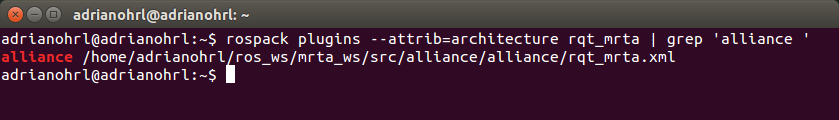
\includegraphics[width=.95\textwidth]{Figuras/4_resultados/rqt_mrta_alliance.png}
                \caption{Ferramenta \textit{rospack} encontra a arquitetura \textit{alliance}.} \label{fig:rospack_alliance}
            \end{figure}
            
            Portanto, verifica-se que o pacote \textit{alliance} está devidamente cadastrado como uma arquitetura disponível para o uso em aplicações através do \textit{plugin rqt\_mrta}.
        
    \section{\textit{patrulha}} \label{sec:patrulha}
        Esta aplicação consiste no patrulhamento realizado por três robôs homogêneos em um ambiente fechado. Foram definidos três comportamentos para cada robô: \textit{wander}, \textit{border\_protection} e \textit{report}. O comportamento \textit{wander} é uma implementação do algoritmo evitador de colisões. O robô permanece avançando para frente até que ele se depara com um anteparo. Sua direção aponta gradativamente para uma direção paralela ao obstáculo com o intuito de evitar uma colisão entre o robô e a parede. O comportamento \textit{border\_protection} implementa um algoritmo seguidor de parede. Através de um controlador P, são comparadas as distâncias aferidas pelos sensores ultrassônicos laterais do robô para mantê-lo dentro de um certo perímetro distante da parede. Enfim, o comportamento \textit{report} é desempenhado pelos robôs de modo a informar ao solicitante da missão sobre o seu progresso.
            
        Com o auxílio do simulador Stage MobileSim\footnote{\url{http://robots.mobilerobots.com/wiki/MobileSim}} da Adept MobileRobots foram utilizados três robôs diferenciais móveis Pioneer 3 DX \cite{ref:adept2011p3dx}, mostrado na Figura \ref{fig:p3_dx}, para simular a dinâmica dos robôs em um ambiente fechado para a simulação de uma aplicação de patrulhamento. Este robô está disponível para uso no Laboratório de Robótica (LRO) da Universidade Federal de Itajubá (UNIFEI). Dado que o foco deste trabalho está na avaliação do pacote \textit{rqt\_mrta}, a aplicação foi simplificada ao máximo, de modo que foram apenas utilizados: (1) o sensor \textit{encoder} para ter uma estimativa do deslocamento do robô, (2) os sensores ultrassônicos para uma estimativa da distância entre o robô e as paredes do ambiente simulado, assim como, (3) seus motores para deslocar o robô pelo ambiente.
        
        \begin{figure}[htb]
            \centering
            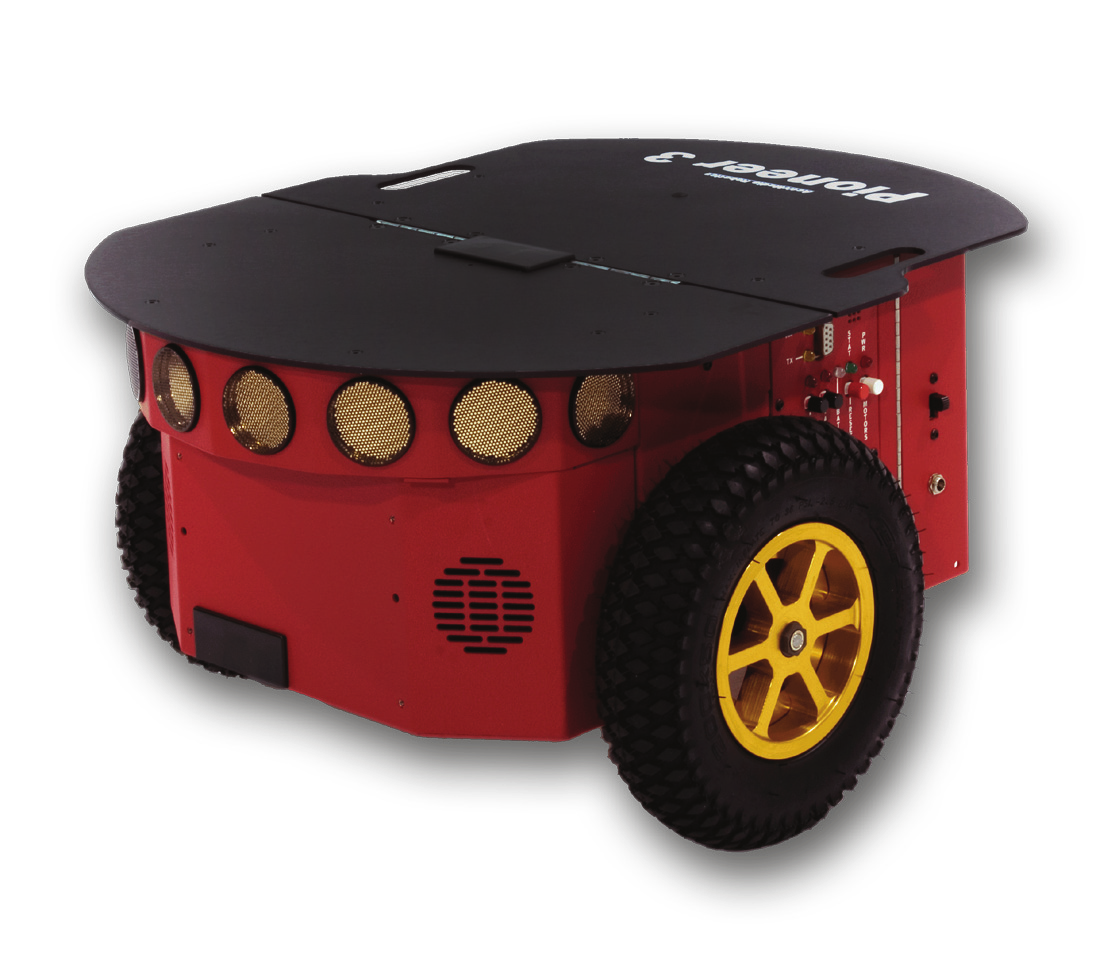
\includegraphics[width=.5\textwidth]{Figuras/4_resultados/p3dx.png}
            \caption[Robô Pioneer 3 DX da Adept MobileRobots.]{Robô Pioneer 3 DX da Adept MobileRobots \cite{ref:adept2011p3dx}.}
            \label{fig:p3_dx}
        \end{figure}
        
        Também foi utilizado o pacote \textit{RosAria}\footnote{\url{http://wiki.ros.org/ROSARIA}} do ROS para ter acesso aos sensores e atuadores dos robôs no ambiente simulado com o sistema de comunicação do ROS através de uma rede de computadores. 
        
        Como é mostrado a seguir, o arquivo de descrição dos \textit{plugin}\footnote{O arquivo de descrição de \textit{plugin} é um arquivo XML que serve para armazenar toda informação importante sobre um \textit{plugin} em um formato legível à máquina. Ele contém informação sobre a biblioteca onde o \textit{plugin} está localizado, seu nome, seu tipo, etc. Para mais informações, vide \url{http://wiki.ros.org/pluginlib}.} desenvolvidos no pacote \textit{alliance\_test} para o pacote \textit{alliance} foram criados para a interação entre a arquitetura ALLIANCE e a aplicação de patrulhamento.
        
        \lstset{
            language=XML,
            basicstyle=\ttfamily,
            keywordstyle=\color{black}\bfseries,
            ndkeywords={},
            ndkeywordstyle=\color{black}\bfseries,
            identifierstyle=\color{black},
            stringstyle=\color{red}\ttfamily,
            commentstyle=\color{green}\ttfamily,
            breaklines=true,
            frameround=ffff,
            frame=single,
            rulecolor=\color{black},
            autogobble=true,
            morekeywords={
                class_libraries,
                    library, path,
                        class, name, type, base_class_type,
                            description,
            }
        }
        
        \begin{lstlisting}
            <class_libraries>
              <library path="lib/liballiance_test">
                <class name="alliance_test/border_protection"
                       type="alliance_test::BorderProtection"
                       base_class_type="alliance::Layer">
                  <description>
                    Border Protection layer for ALLIANCE MRTA architecture.
                  </description>
                </class>
                <class name="alliance_test/report"
                       type="alliance_test::Report"
                       base_class_type="alliance::Layer">
                  <description>
                    Report layer for ALLIANCE MRTA architecture.
                  </description>
                </class>
                <class name="alliance_test/wander"
                       type="alliance_test::Wander"
                       base_class_type="alliance::Layer">
                  <description>
                    Wander layer for ALLIANCE MRTA architecture.
                  </description>
                </class>
                <class name="alliance_test/odometry"
                       type="alliance_test::Odometry"
                       base_class_type="alliance::Sensor">
                  <description>
                    nav_msgs/Odometry message wrapper for sensor data receiving.
                  </description>
                </class>
                <class name="alliance_test/point_cloud"
                       type="alliance_test::PointCloud"
                       base_class_type="alliance::Sensor">
                  <description>
                    sensor_msgs/PointCloud message wrapper for sensor data receiving.
                  </description>
                </class>
                <class name="alliance_test/updated_sensory"
                       type="alliance_test::UpdatedSensory"
                       base_class_type="alliance::SensoryEvaluator">
                  <description>
                    This evaluator verifies if all sensors are up-to-date.
                  </description>
                </class>
              </library>
            </class_libraries>
        \end{lstlisting}
    
        \subsection{Criação da aplicação através do \textit{plugin rqt\_mrta}} \label{subsec:criacao_patrulha}
            Para a criação da aplicação \textit{patrulha}, foi utilizado o \textit{wizard} de criação de aplicações do \textit{plugin rqt\_mrta} descrito em \ref{subsec:rqt_mrta_view}. A Figura \ref{fig:patrulha_new_app} exibe as telas do \textit{wizard} de criação de aplicação do \textit{rqt\_mrta} devidamente preenchidas.
        
            \begin{figure}[htb]
                \centering
                \subfloat[Dados gerais da aplicação.]{
                    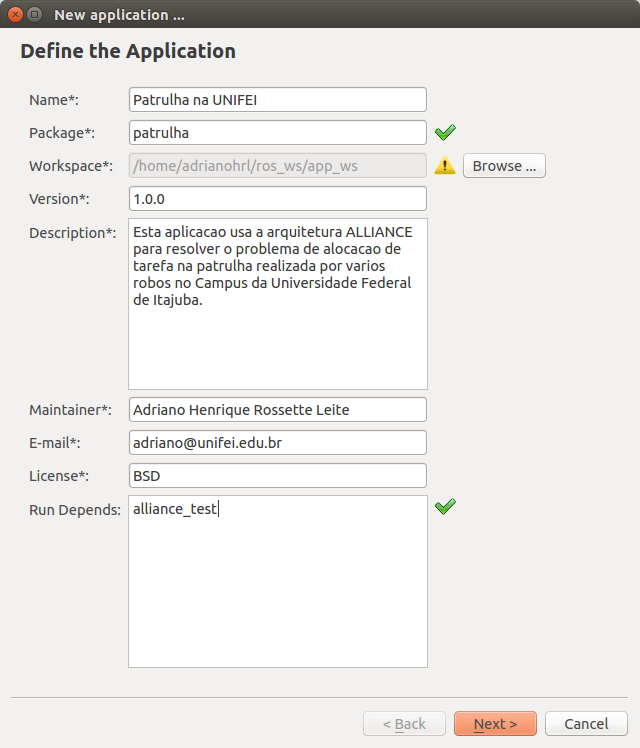
\includegraphics[width=.31\textwidth]{Figuras/4_resultados/patrulha_def_app.png}
                    \label{fig:patrulha_def_app}
                }
                \subfloat[Escolha da arquitetura.]{
                    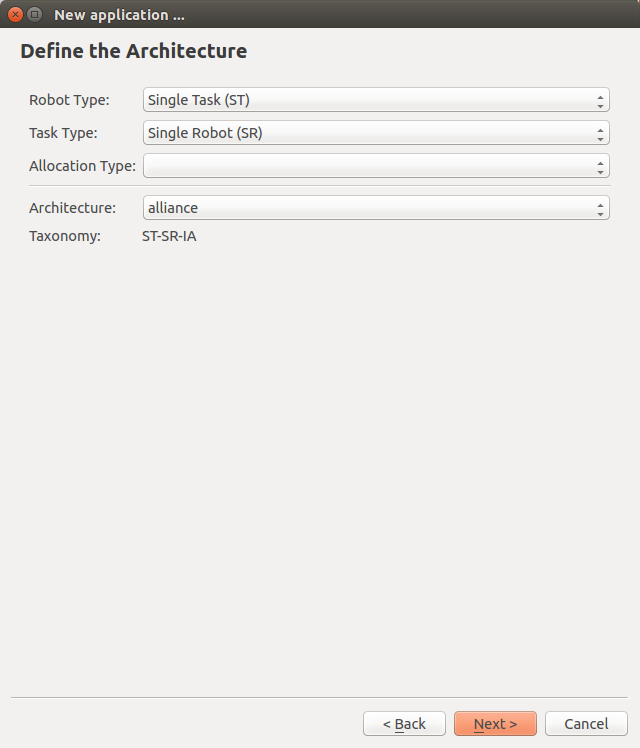
\includegraphics[width=.31\textwidth]{Figuras/4_resultados/patrulha_def_arch.png}
                    \label{fig:patrulha_def_arch}
                }
                \subfloat[Definição dos robôs do sistema.]{
                    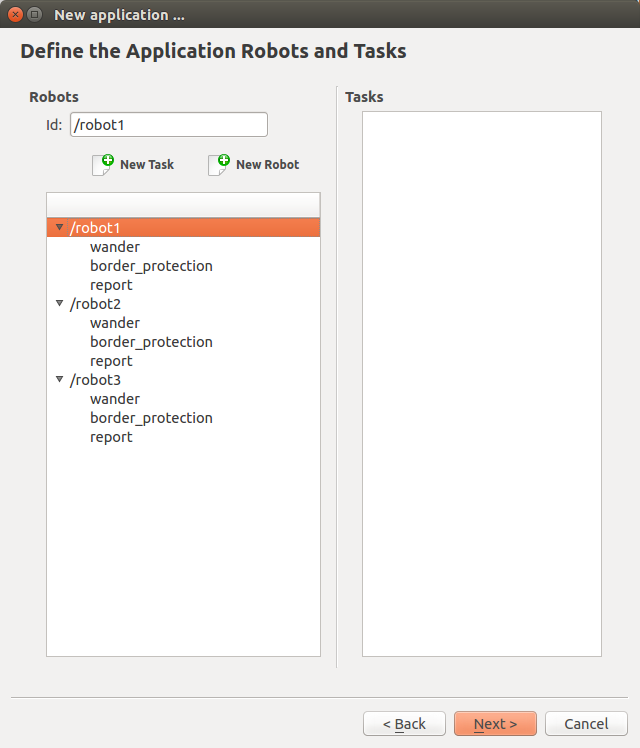
\includegraphics[width=.31\textwidth]{Figuras/4_resultados/patrulha_def_robots.png}
                    \label{fig:patrulha_def_robots}
                }
                
                \subfloat[Parametrização da arquitetura.]{
                    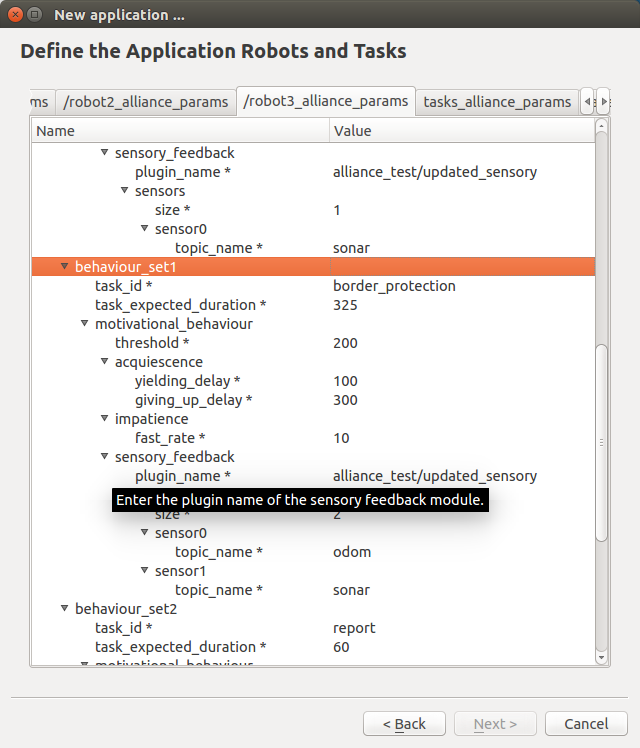
\includegraphics[width=.31\textwidth]{Figuras/4_resultados/patrulha_def_params.png}
                    \label{fig:patrulha_def_params}
                }
                \subfloat[Sumário.]{
                    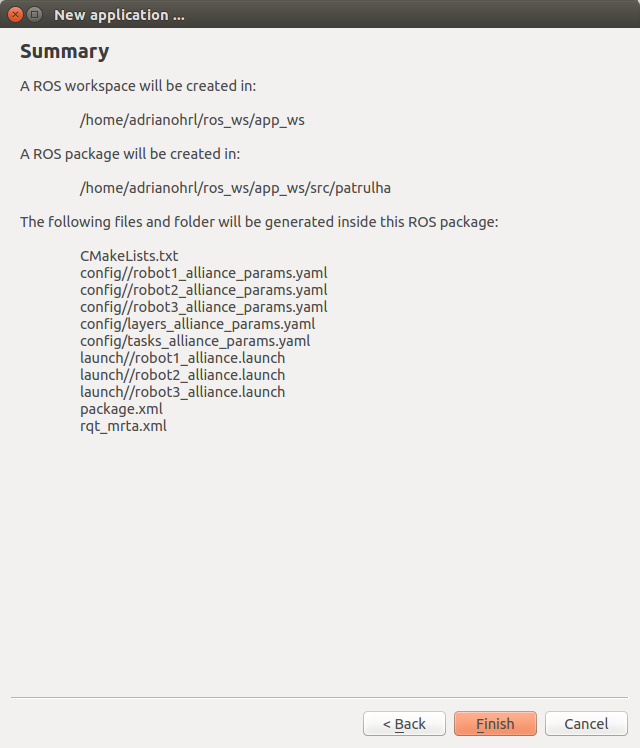
\includegraphics[width=.31\textwidth]{Figuras/4_resultados/patrulha_summary.png}
                    \label{fig:patrulha_summary}
                }
                \caption{Criação da aplicação \textit{patrulha}.} \label{fig:patrulha_new_app}
            \end{figure}
            
            Primeiramente, foram preenchidos os dados referentes a criação do pacote da aplicação (vide Figura \ref{fig:patrulha_def_app}). Nesta etapa, foram inseridos: (1) o nome da aplicação, (2) o nome do pacote da aplicação, (3) o diretório do \textit{workspace} em que o pacote foi criado, (4) a versão do pacote, (5) a descrição da aplicação, (6) o nome do mantenedor do pacote da aplicação e (7) seu \textit{e-mail}, (8) o tipo de licença do pacote e (9) a dependência em tempo de execução do pacote \textit{alliance\_test}, que implementa os \textit{plugins} necessários para o controle da execução das tarefas da aplicação \textit{patrulha}. Como o diretório do \textit{workspace} fornecido não era um \textit{workspace} do ROS, um alerta foi gerado, informando que este diretório seria transformado em um \textit{workspace} do ROS.
            
            Em seguida, foi selecionada a arquitetura \textit{alliance} (vide Figura \ref{fig:patrulha_def_arch}). Lembrando que, se o usuário não souber qual arquitetura ele irá usar, este pode utilizar os filtros de acordo com a classificação da taxonomia de \cite{ref:gerkey2004taxonomy} para o seu problema MRTA. 
            
            Na sequência, foi solicitado o preenchimento dos robôs do sistema (vide Figura \ref{fig:patrulha_def_robots}). Os três robôs foram inseridos: (1) \textit{/robot1}, (2) \textit{/robot2} e (3) \textit{/robot3}. Como este é um sistema homogêneo, todos os robôs podem executar as três tarefas do problema: (1) \textit{wander}, (2) \textit{border\_protection} e (3) \textit{report}.
            
            Foram preenchidas, na próxima tela (vide Figura \ref{fig:patrulha_def_params}), os parâmetros para cinco arquivos de parâmetros: um para cada robô, uma para as tarefas e um para as camadas. Assim que todos parâmetros obrigatórios foram preenchidos, o botão \textit{Next} se tornou habilitado. 
            
            Na última tela do \textit{wizard} (vide Figura \ref{fig:patrulha_summary}), foi exibida uma mensagem resumindo o que aconteceria ao pressionar o botão \textit{Finish}. Foi dito que: 
            
            \begin{itemize}
                \item seria iniciado um \textit{workspace} do ROS no diretório dado;
                \item seria criado um pacote ROS no diretório \textit{src} do \textit{workspace};
                \item seriam gerados os arquivos \textit{CMakeLists.txt}, \textit{package.xml} e \textit{rqt\_mrta.xml} na raiz do pacote;
                \item seriam gerados os cinco arquivos de parâmetros (de extensão \textit{.yaml}) dentro da pasta \textit{config} do pacote;
                \item e seriam gerados os três arquivos de inicialização (de extensão \textit{.launch}) dentro da pasta \textit{launch} do pacote.
            \end{itemize}
            
        \subsection{Análise da aplicação gerada} \label{subsec:analise_patrulha}
            Ao pressionar o botão \textit{Finish} do \textit{wizard} de criação de aplicação, todos as pastas e arquivos citados acima foram criadas e gerados, respectivamente. A Figura \ref{fig:patrulha} mostra a estrutura do pacote \textit{patrulha} criado.
            
            \begin{figure}[htb]
                \centering
                \subfloat[Pacote.]{
                    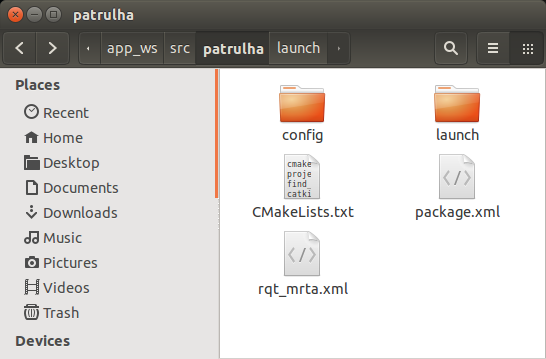
\includegraphics[width=.4\textwidth]{Figuras/4_resultados/patrulha_pkg.png}
                    \label{fig:patrulha_pkg}
                }
                \subfloat[Arquivos de parâmetro.]{
                    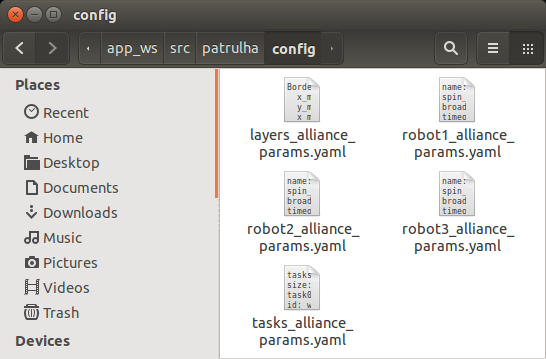
\includegraphics[width=.4\textwidth]{Figuras/4_resultados/patrulha_pkg_config.png}
                    \label{fig:patrulha_pkg_config}
                }
                
                \subfloat[Arquivos de inicialização.]{
                    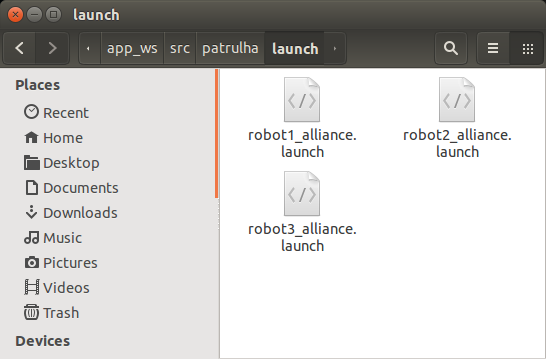
\includegraphics[width=.4\textwidth]{Figuras/4_resultados/patrulha_pkg_launch.png}
                    \label{fig:patrulha_pkg_launch}
                }
                \caption{Pastas e arquivos gerados após a criação de uma aplicação.} \label{fig:patrulha}
            \end{figure}
        
            Observa-se que o pacote está devidamente organizado, agrupando os arquivos de parâmetros na pasta \textit{config} e os arquivos de inicialização na pasta \textit{launch}. Além disso, verificou-se que os arquivos gerados, possuem a formatação esperada. Os Apêndices \ref{app:app_config} e \ref{app:app_manifest} mostram os arquivos de configuração de aplicação e de manifesto do pacote \textit{patrulha} gerados.
        
            Para verificar se o pacote \textit{patrulha} foi configurado como uma aplicação do ponto de vista do \textit{plugin rqt\_mrta}, foi usada a ferramenta \textit{rospack plugin}, só que desta vez, passando como atributo \textit{application}. Como foi dito anteriormente, esta mesma ferramenta é utilizada pelo \textit{rqt\_mrta} para procurar as aplicações e arquiteturas no sistema de arquivos do ROS. O resultado deste comando pode ser visualizado na Figura \ref{fig:rospack_patrulha}.
        
            \begin{figure}[htb]
                \centering
                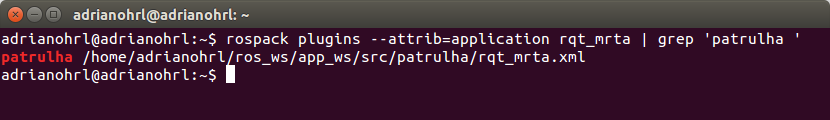
\includegraphics[width=.95\textwidth]{Figuras/4_resultados/rqt_mrta_patrulha.png}
                \caption{Ferramenta \textit{rospack} encontra a aplicação \textit{patrulha}.} \label{fig:rospack_patrulha}
            \end{figure}
            
            Portanto, verifica-se que o pacote \textit{patrulha} está devidamente cadastrado como uma aplicação no ponto de vista do \textit{plugin rqt\_mrta}.
            
        \subsection{Simulação a partir dos arquivos gerados} \label{subsec:sim_patrulha}
            Cabe agora a validação dos arquivos gerados através da execução dos arquivos de inicialização gerados através da ferramenta \textit{roslaunch}. 
            
            A Figura \ref{fig:patrulha_launches} exibe cinco terminais enumerados de 1 à 5. O Terminal 1 mostra as saídas do comando de linha \textit{rosnode list} que mostra os nós em execução no ROS. Este comando foi executado antes e após a inicialização dos nós da arquitetura de cada robô. Logo, verifica-se que inicialmente apenas o nó mestre do ROS que está em execução. Após a inicialização dos nós do robô \textit{/robot1} (vide Terminal 3), os nós \textit{/robot1/alliance/low\_level} e \textit{/robot1/alliance/high\_level} passaram a executar juntamente com o nó mestre do ROS. No Terminal 4, ao inicializar os nós do robô \textit{/robot2}, os nós \textit{low\_level} e \textit{high\_level} com o \textit{namespace /robot2/alliance} passaram a executar juntamente com os demais. Por fim, no Terminal 5, ao executar o comando \textit{roslaunch} para o arquivo de inicialização do robô \textit{/robot3}, os nós \textit{low\_level} e \textit{high\_level} com o \textit{namespace /robot3/alliance} passaram a executar juntamente com os demais. O Terminal 2 lista os tópicos existentes no ROS após a inicialização de todos os nós citados acima.
            
            \begin{figure}[htb]
                \centering
                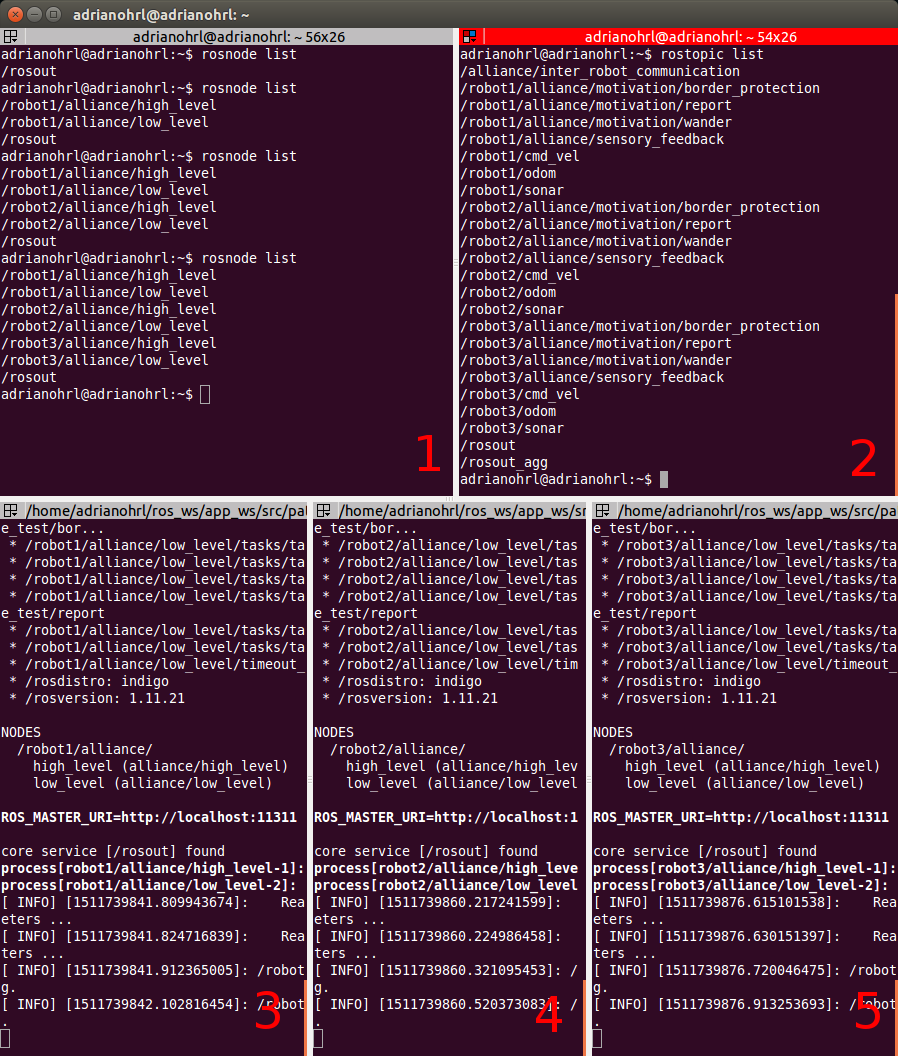
\includegraphics[width=.97\textwidth]{Figuras/4_resultados/patrulha_launches.png}
                \caption{Inicialização dos nós da arquitetura para três robôs.} \label{fig:patrulha_launches}
            \end{figure}
            
            Outra forma de visualizar a execução correta dos nós da arquitetura do pacote \textit{alliance} para a aplicação \textit{patrulha} pode ser vista com mais detalhes na Figura \ref{fig:patrulha_rosgraph}. Esta figura foi extraída da ferramenta \textit{rqt\_graph}\footnote{\url{http://wiki.ros.org/rqt_graph}} disponível no ROS, onde nós são representados por elipses e tópicos são representados por retângulos.
        
            \begin{figure}[htb]
                \centering
                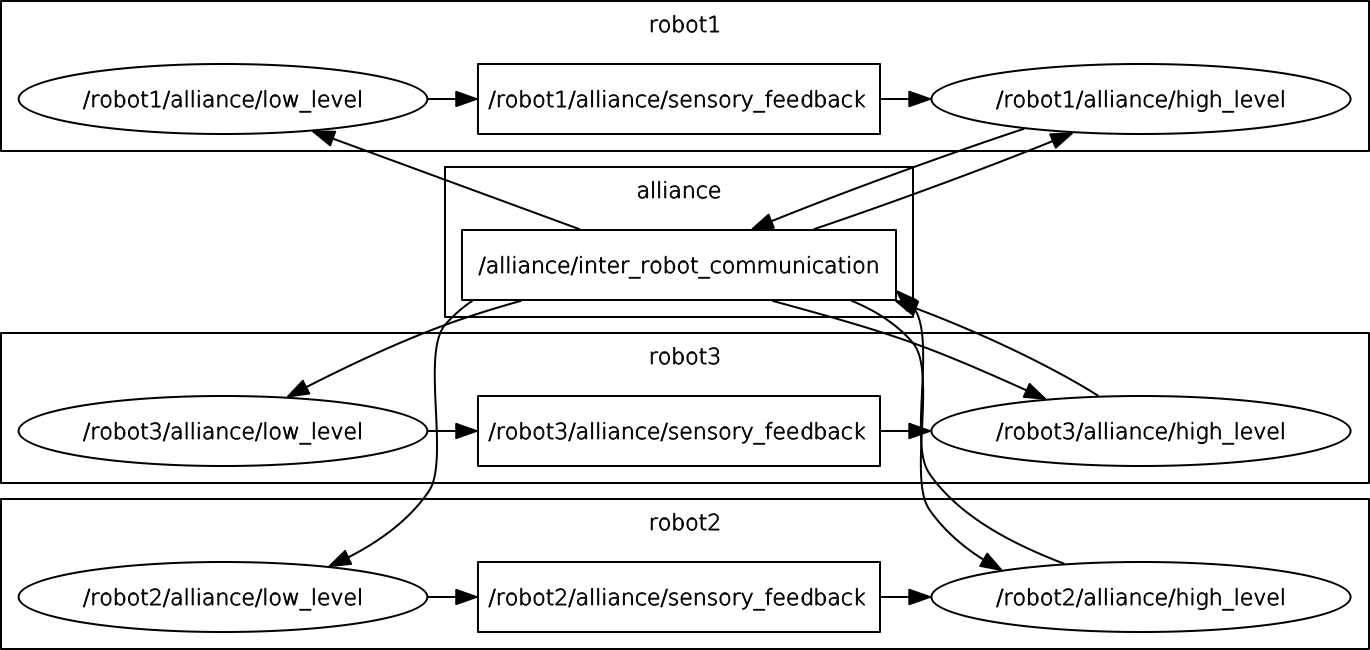
\includegraphics[width=.75\textwidth]{Figuras/4_resultados/alliance_rosgraph.png}
                \caption{Grafo da arquitetura \textit{alliance} no ROS para três robôs.} \label{fig:alliance_rosgraph}
            \end{figure}
        
            Entretanto, até o presente momento, apenas a arquitetura está sendo executada juntamente com o camada de controle de execução das tarefas. Torna-se, ainda, necessário adicionar os robôs ao sistema. Pois os sinais providos dos seus sensores são inexistentes. Além disso, não existem atuadores para serem comandados.
            
            Conforme é exibido na Figura \ref{fig:patrulha_rosgraph}, ao executar todos os nós necessários para a aplicação \textit{patrulha}, verifica-se que o nó \textit{alliance/low\_level} interage diretamente com o nó \textit{RosAria} dentro do \textit{namespace} de cada robô (\textit{/robot1}, \textit{robot2} e \textit{/robot3}). Observa-se que, para cada \textit{namespace}, o nó \textit{alliance/low\_level} publica no tópico \textit{cmd\_vel} e está inscrito nos tópicos \textit{odom} e \textit{sonar}; enquanto que o nó \textit{RosAria} subscreve o tópico \textit{cmd\_vel} e publica nos tópicos \textit{odom} e \textit{sonar}. Isso acontecido devido à subscrições e publicações realizadas pelos \textit{plugins} carregados nos nós \textit{alliance/low\_level} de cada \textit{namespace}. Para cada \textit{namespace}, os tópicos:
            
            \begin{itemize}
                \item \textit{odom} disponibiliza a informação de odometria do robô;
                
                \item \textit{sonar} disponibiliza os sinais dos sensores ultrassônicos do robô;
                
                \item e, por fim, \textit{cmd\_vel} disponibiliza o comando de velocidade do robô.
            \end{itemize}
        
            \begin{figure}[p]
                \centering
                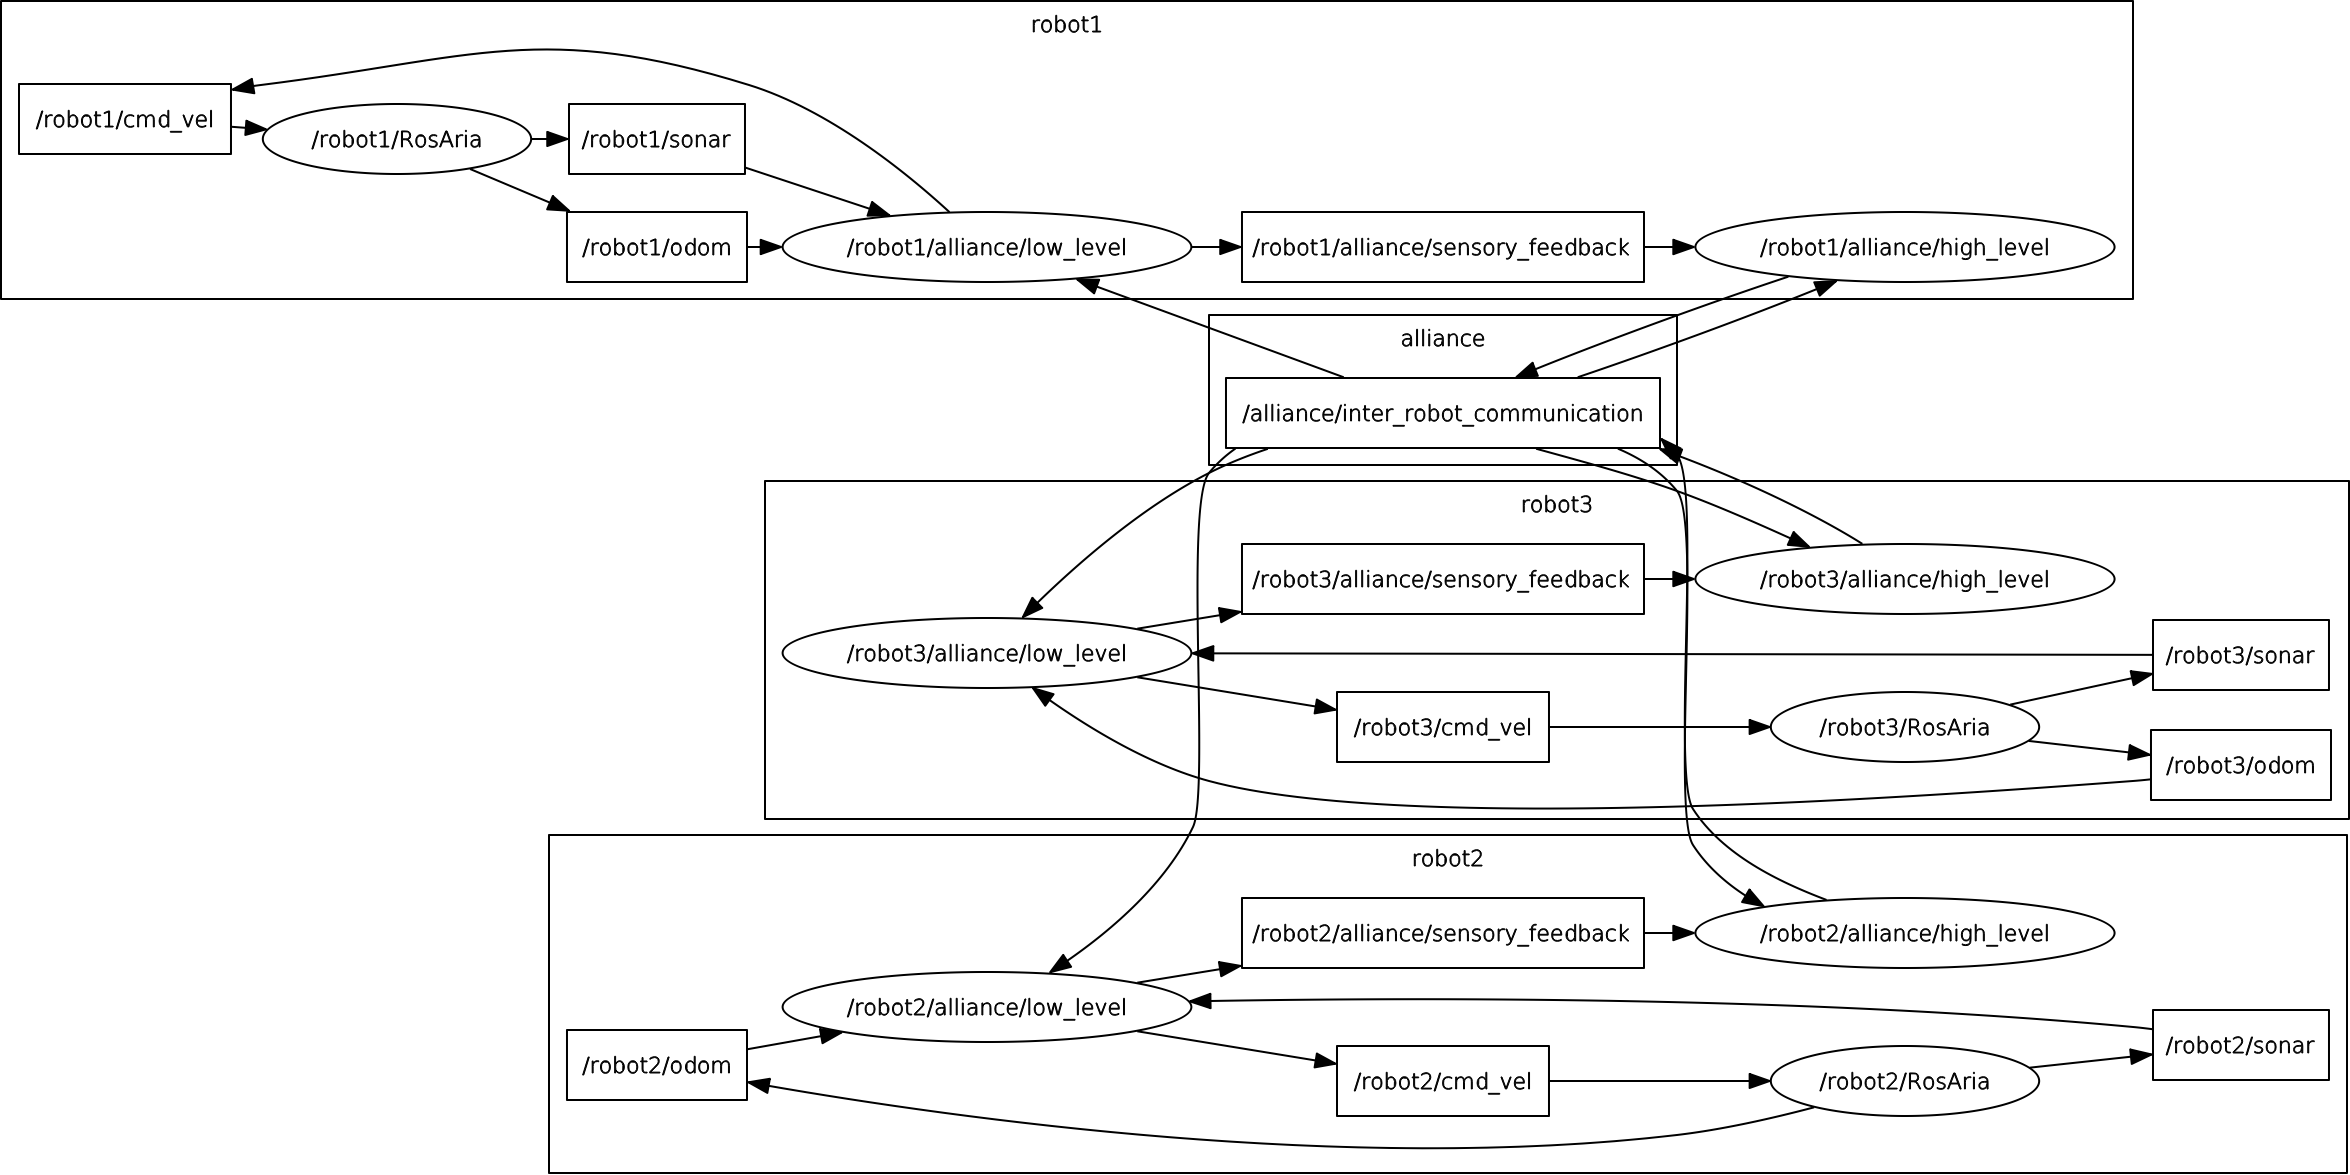
\includegraphics[width=.95\textheight,angle=90]{Figuras/4_resultados/patrulha_rosgraph.png}
                \caption{Grafo da aplicação \textit{patrulha} no ROS.} \label{fig:patrulha_rosgraph}
            \end{figure}
            
        \subsection{Supervisão}
            O \textit{plugin rqt\_mrta} também fornece elementos gráficos para a supervisão da aplicação em tempo de execução. E, caso a arquitetura escolhida fornece ferramentas para a sua análise, o \textit{plugin} as 
        
            \begin{figure}[p]
                \centering
                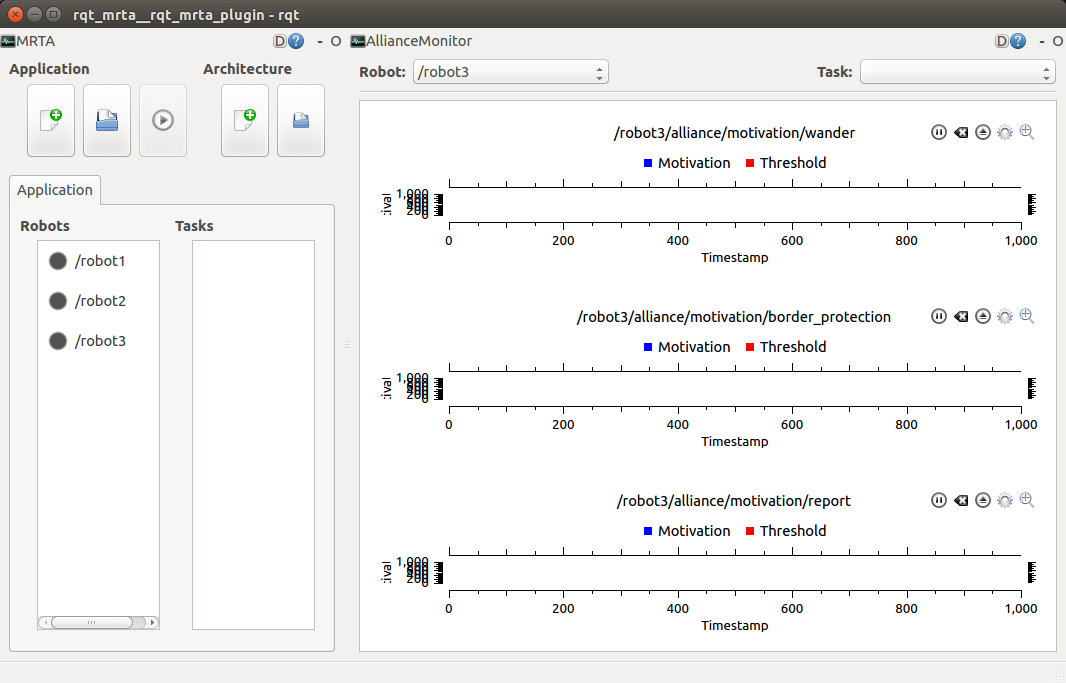
\includegraphics[width=.75\textwidth]{Figuras/4_resultados/rqt_mrta1.png}
                \caption{Grafo da aplicação \textit{patrulha} no ROS.} \label{fig:rqt_mrta1}
            \end{figure}
        
            \begin{figure}[p]
                \centering
                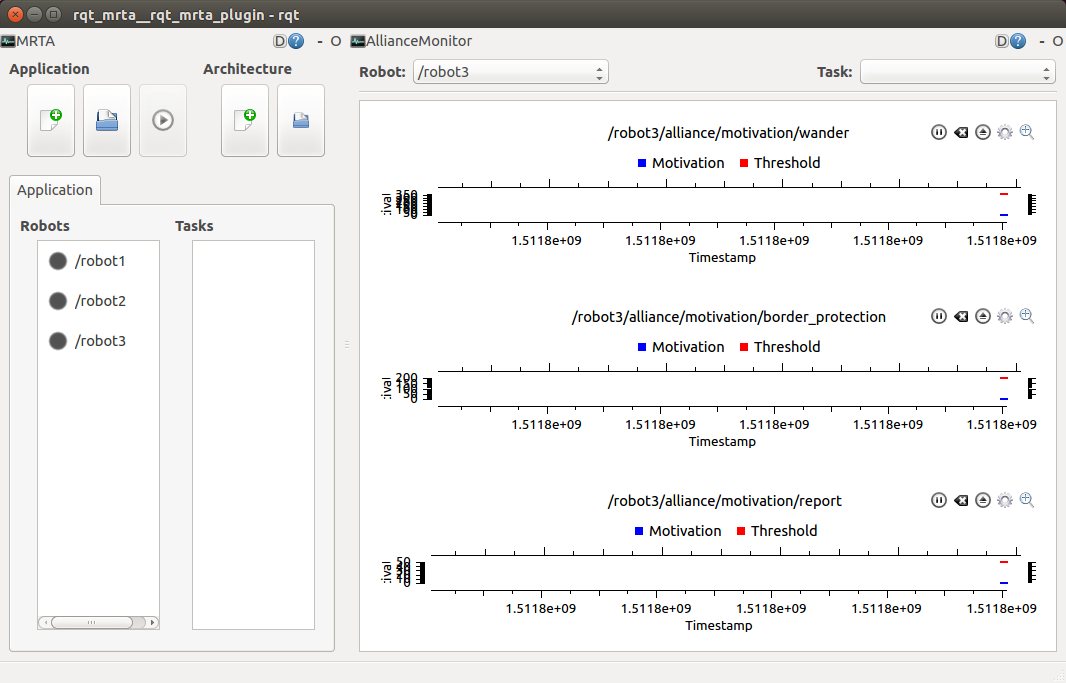
\includegraphics[width=.75\textwidth]{Figuras/4_resultados/rqt_mrta2.png}
                \caption{Grafo da aplicação \textit{patrulha} no ROS.} \label{fig:rqt_mrta2}
            \end{figure}
        
            \begin{figure}[p]
                \centering
                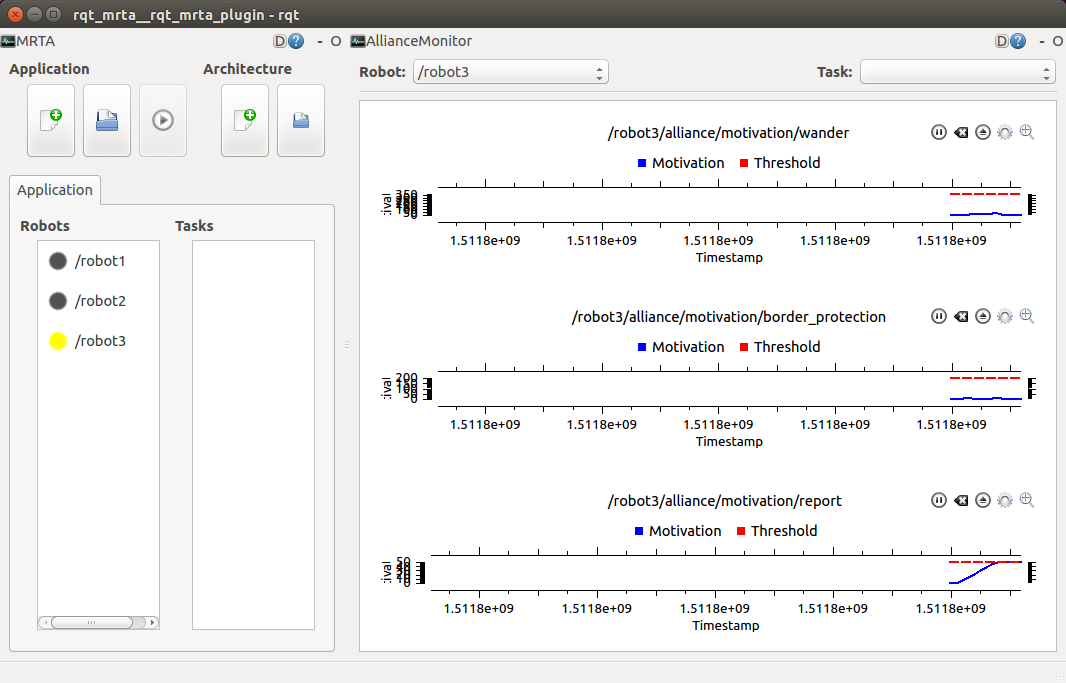
\includegraphics[width=.75\textwidth]{Figuras/4_resultados/rqt_mrta3.png}
                \caption{Grafo da aplicação \textit{patrulha} no ROS.} \label{fig:rqt_mrta3}
            \end{figure}
        
            \begin{figure}[p]
                \centering
                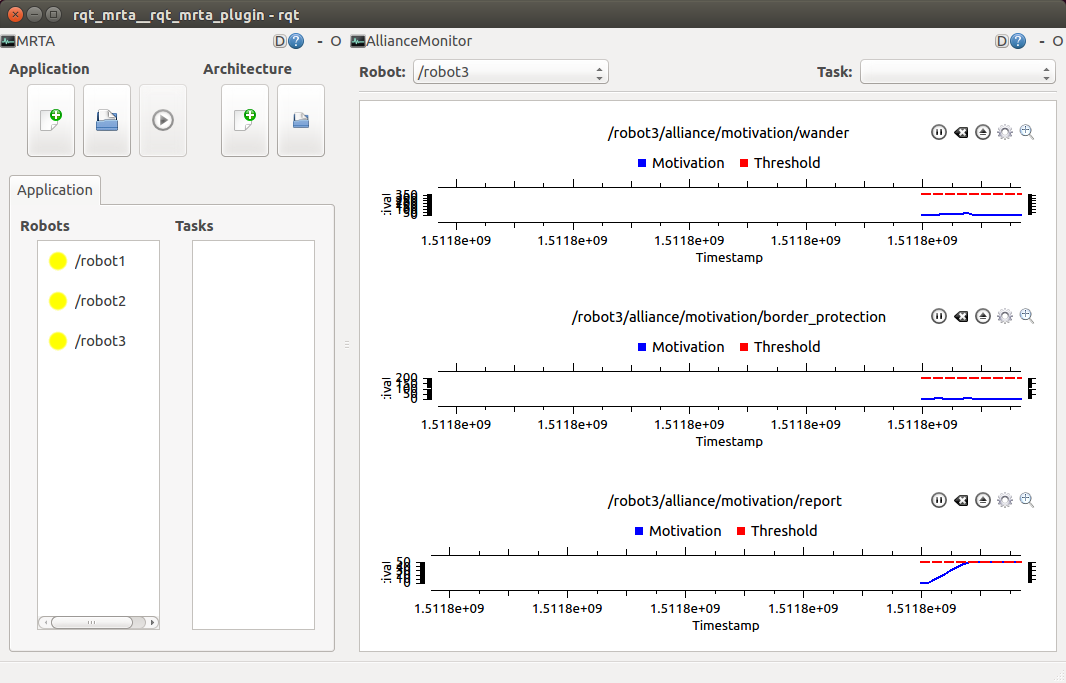
\includegraphics[width=.75\textwidth]{Figuras/4_resultados/rqt_mrta4.png}
                \caption{Grafo da aplicação \textit{patrulha} no ROS.} \label{fig:rqt_mrta4}
            \end{figure}
        
            \begin{figure}[p]
                \centering
                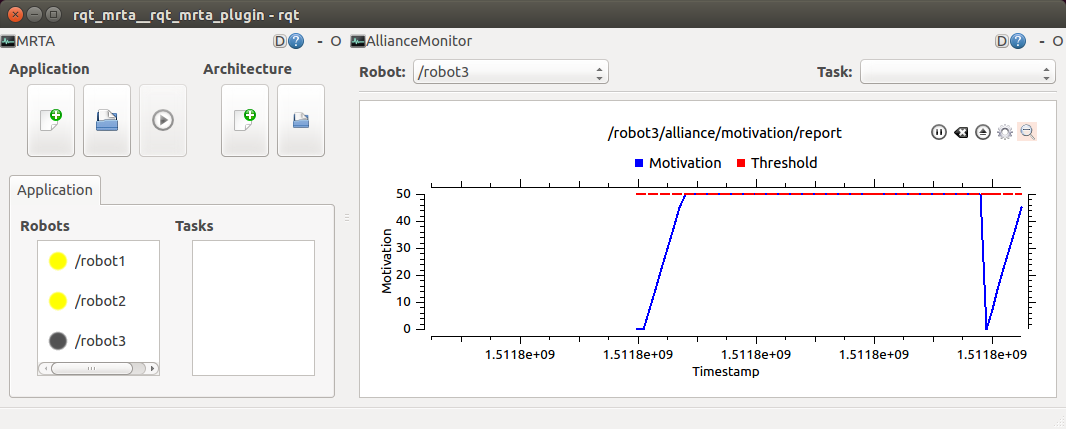
\includegraphics[width=.75\textwidth]{Figuras/4_resultados/rqt_mrta5.png}
                \caption{Grafo da aplicação \textit{patrulha} no ROS.} \label{fig:rqt_mrta5}
            \end{figure}
            
            \begin{figure}[htb]
                \centering
                \subfloat[Arquivos de parâmetro.]{
                    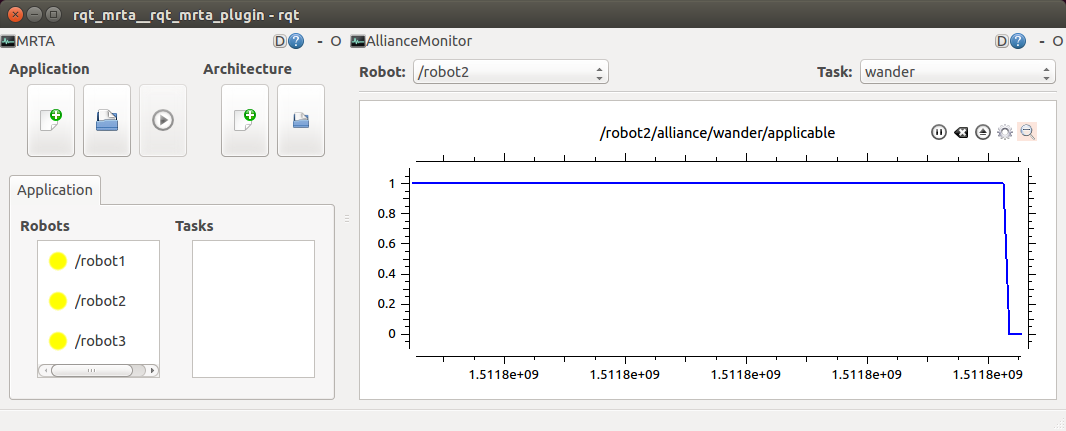
\includegraphics[width=.75\textwidth]{Figuras/4_resultados/rqt_mrta6.png}
                    \label{fig:rqt_mrta6}
                }
                
                \subfloat[Arquivos de inicialização.]{
                    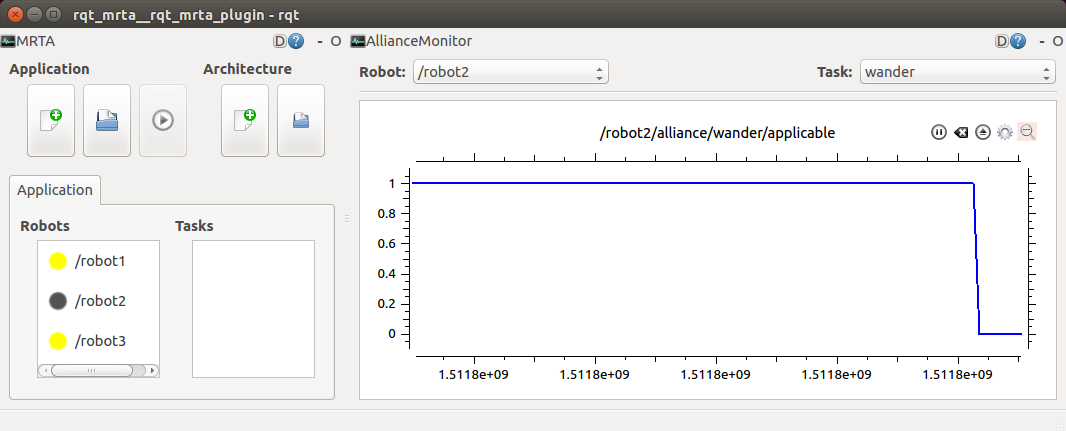
\includegraphics[width=.75\textwidth]{Figuras/4_resultados/rqt_mrta7.png}
                    \label{fig:rqt_mrta7}
                }
                
                \subfloat[Arquivos de inicialização.]{
                    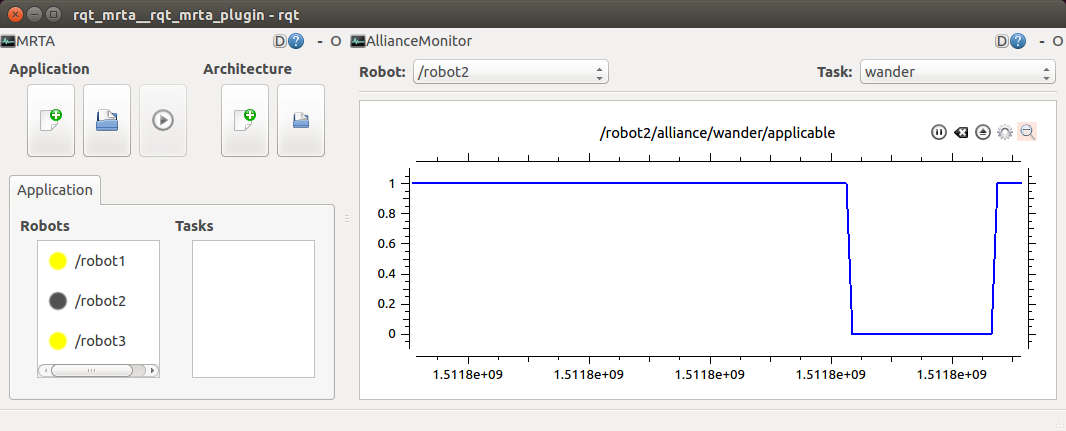
\includegraphics[width=.75\textwidth]{Figuras/4_resultados/rqt_mrta8.png}
                    \label{fig:rqt_mrta8}
                }
                
                \subfloat[Arquivos de inicialização.]{
                    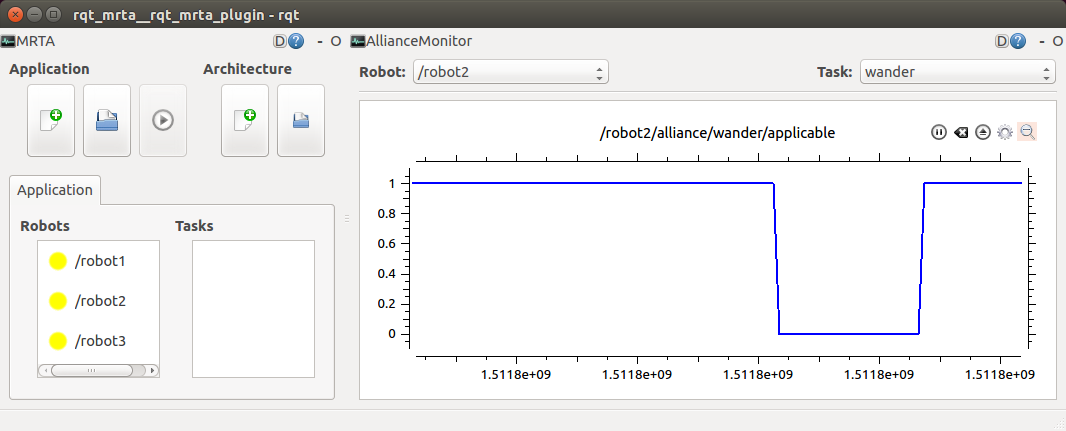
\includegraphics[width=.75\textwidth]{Figuras/4_resultados/rqt_mrta9.png}
                    \label{fig:rqt_mrta9}
                }
                \caption{Pastas e arquivos gerados após a criação de uma aplicação.} \label{fig:patrulha_rqt_mrta}
            \end{figure}
        
    
        %\pgfplotstableread[col sep=comma]{\detokenize{Figuras/capitulo_3/robot1-wander-motivation-new.csv}}\datatable
\begin{figure}[htb]
    \centering
    \begin{tikzpicture}
    \begin{groupplot}[
      group style={rows=6}, 
      width=0.75\textwidth,
      height=0.25\textwidth, 
      xmajorgrids, 
      ymajorgrids, 
      enlarge x limits=false,
    ] 
        \nextgroupplot[
        %title={Motivação da configuração de comportamento /robot1/wander.},
        ymin=-0.1,
        ylabel={$impaci\hat{e}ncia(t)$},
        ]
        \addplot[blue,line width=1pt] table[x index=0,y index=1]{\datatable}; 
        
        \nextgroupplot[
        ymin=-0.1,
        ymax=1.1,
        ylabel={$aquiescente(t)$},
        ] 
        \addplot[blue,line width=1pt] table[x index=0,y index=2]{\datatable}; 
        
        \nextgroupplot[
        ymin=-0.1,
        ymax=1.1,
        ylabel={$inibida(t)$},
        ] 
        \addplot[blue,line width=1pt] table[x index=0,y index=3]{\datatable}; 
        
        \nextgroupplot[
        ymin=-0.1,
        ymax=1.1,
        ylabel={$reiniciada(t)$},
        ] 
        \addplot[blue,line width=1pt] table[x index=0,y index=4]{\datatable}; 
        
        \nextgroupplot[
        ymin=-0.1,
        ymax=1.1,
        ylabel={$aplic\acute{a}vel(t)$},
        ] 
        \addplot[blue,line width=1pt] table[x index=0,y index=5]{\datatable};
        
        \nextgroupplot[
        ylabel={$motiva\textit{ç}\tilde{a}o(t)$},
        xlabel={$t [s]$}
        ] 
        \addplot[blue,line width=1pt] table[x index=0,y index=6]{\datatable};
    \end{groupplot}
\end{tikzpicture}
    \caption{Motivação da configuração de comportamento /robot1/wander.} \label{fig:motivacao1}
\end{figure}

\pgfplotstableread[col sep=comma]{\detokenize{Figuras/capitulo_3/robot2-wander-motivation-new.csv}}\datatable
\begin{figure}[htb]
    \centering
    \begin{tikzpicture}
    \begin{groupplot}[
      group style={rows=6}, 
      width=0.75\textwidth,
      height=0.25\textwidth, 
      xmajorgrids, 
      ymajorgrids, 
      enlarge x limits=false,
    ] 
        \nextgroupplot[
        %title={Motivação da configuração de comportamento /robot1/wander.},
        ymin=-0.1,
        ylabel={$impaci\hat{e}ncia(t)$},
        ]
        \addplot[blue,line width=1pt] table[x index=0,y index=1]{\datatable}; 
        
        \nextgroupplot[
        ymin=-0.1,
        ymax=1.1,
        ylabel={$aquiescente(t)$},
        ] 
        \addplot[blue,line width=1pt] table[x index=0,y index=2]{\datatable}; 
        
        \nextgroupplot[
        ymin=-0.1,
        ymax=1.1,
        ylabel={$inibida(t)$},
        ] 
        \addplot[blue,line width=1pt] table[x index=0,y index=3]{\datatable}; 
        
        \nextgroupplot[
        ymin=-0.1,
        ymax=1.1,
        ylabel={$reiniciada(t)$},
        ] 
        \addplot[blue,line width=1pt] table[x index=0,y index=4]{\datatable}; 
        
        \nextgroupplot[
        ymin=-0.1,
        ymax=1.1,
        ylabel={$aplic\acute{a}vel(t)$},
        ] 
        \addplot[blue,line width=1pt] table[x index=0,y index=5]{\datatable};
        
        \nextgroupplot[
        ylabel={$motiva\textit{ç}\tilde{a}o(t)$},
        xlabel={$t [s]$}
        ] 
        \addplot[blue,line width=1pt] table[x index=0,y index=6]{\datatable};
    \end{groupplot}
\end{tikzpicture}
    \caption{Motivação da configuração de comportamento /robot2/wander.} \label{fig:motivacao2}
\end{figure}

\pgfplotstableread[col sep=comma]{\detokenize{Figuras/capitulo_3/robot2-border-protection-motivation-new.csv}}\datatable
\begin{figure}[htb]
    \centering
    \begin{tikzpicture}
    \begin{groupplot}[
      group style={rows=6}, 
      width=0.75\textwidth,
      height=0.25\textwidth, 
      xmajorgrids, 
      ymajorgrids, 
      enlarge x limits=false,
    ] 
        \nextgroupplot[
        %title={Motivação da configuração de comportamento /robot1/wander.},
        ymin=-0.1,
        ylabel={$impaci\hat{e}ncia(t)$},
        ]
        \addplot[blue,line width=1pt] table[x index=0,y index=1]{\datatable}; 
        
        \nextgroupplot[
        ymin=-0.1,
        ymax=1.1,
        ylabel={$aquiescente(t)$},
        ] 
        \addplot[blue,line width=1pt] table[x index=0,y index=2]{\datatable}; 
        
        \nextgroupplot[
        ymin=-0.1,
        ymax=1.1,
        ylabel={$inibida(t)$},
        ] 
        \addplot[blue,line width=1pt] table[x index=0,y index=3]{\datatable}; 
        
        \nextgroupplot[
        ymin=-0.1,
        ymax=1.1,
        ylabel={$reiniciada(t)$},
        ] 
        \addplot[blue,line width=1pt] table[x index=0,y index=4]{\datatable}; 
        
        \nextgroupplot[
        ymin=-0.1,
        ymax=1.1,
        ylabel={$aplic\acute{a}vel(t)$},
        ] 
        \addplot[blue,line width=1pt] table[x index=0,y index=5]{\datatable};
        
        \nextgroupplot[
        ylabel={$motiva\textit{ç}\tilde{a}o(t)$},
        xlabel={$t [s]$}
        ] 
        \addplot[blue,line width=1pt] table[x index=0,y index=6]{\datatable};
    \end{groupplot}
\end{tikzpicture}
    \caption{Motivação da configuração de comportamento /robot2/border-protection.} \label{fig:motivacao3}
\end{figure}